\documentclass{../../templates/lkx_pset}

\title{Astron 140 Final}
\author{Lev Kruglyak}
\due{December 16, 2024}

\usepackage{mdframed}


\usepackage[T1]{fontenc}
\RequirePackage{mlmodern}


\mdfdefinestyle{answer}{%
	linecolor=black,
	outerlinewidth=2pt,
	%roundcorner=20pt,
	innertopmargin=4pt,
	innerbottommargin=4pt,
	innerrightmargin=4pt,
	innerleftmargin=4pt,
	leftmargin = 4pt,
	rightmargin = 4pt
	%backgroundcolor=gray!50!white}
}

\newenvironment{answerbox}{
	\begin{mdframed}[style=answer,nobreak=true,userdefinedwidth=30em]}{\end{mdframed}}

\usepackage{siunitx}
\providecommand{\unitsi}[1]{\qty[per-mode = symbol]{#1}{}}
\providecommand{\mpssi}[1]{\qty[per-mode = symbol]{#1}{\m\per\s}}
\providecommand{\mpsssi}[1]{\qty[per-mode = symbol]{#1}{\m\per\s^2}}
\providecommand{\Gsi}[1]{\qty[per-mode = symbol]{#1}{\m^3\per\s^2\kg}}
\providecommand{\kBsi}[1]{\qty[per-mode = symbol]{#1}{\m^2\s^{-2}\K^{-1}\kg}}
\providecommand{\hsi}[1]{\qty[per-mode = symbol]{#1}{\J\cdot s}}
\providecommand{\kgsi}[1]{\qty[per-mode = symbol]{#1}{\kg}}
\providecommand{\ssi}[1]{\qty[per-mode = symbol]{#1}{\s}}
\providecommand{\psssi}[1]{\qty[per-mode = symbol]{#1}{\s^{-2}}}
\providecommand{\msi}[1]{\qty[per-mode = symbol]{#1}{\m}}
\providecommand{\desi}[1]{\qty[per-mode = symbol]{#1}{\J\per \m^3}}

\renewcommand{\O}{\mathrm{O}}
\providecommand{\Aff}{\mathrm{Aff}}
\providecommand{\SO}{\mathrm{SO}}

\providecommand{\Frame}{\mathrm{Fr}}

\providecommand{\A}{\mathbb{A}}

\providecommand{\definefunction}[5]{
	\begin{array}{rcl}
		#1 : #2 & \xrightarrow{\phantom{---}} & #3 \\
		#4      & \xmapsto{\phantom{---}}     & #5
	\end{array}
}


\providecommand{\pp}[2]{\frac{\partial #1}{\partial #2}}


\renewcommand{\abstractname}{Honor Code Statement}
\begin{document}
\maketitle

\vfill
\begin{abstract}
I affirm my awareness of the standards of the Harvard College Honor Code. While completing this exam, I have not consulted any external sources other than class notes and the textbooks. I have not discussed the problems or solutions of this exam with anyone, and will not discuss them until after the due date.

\medskip
Signed, \underline{\textit{Lev Kruglyak}}.
\end{abstract}
\vfill

\pagebreak
\begin{problem}{1}[Gravitational Waves]
\end{problem}
\begin{parts}
  \begin{part}{(a)}
    To study gravitational waves we perturbed the metric around flat spacetime as $g_{\mu\nu} = \eta_{\mu\nu} + h_{\mu\nu}$ and expanded the Riemann tensor up to the first order in $h_{\mu\nu}$. Show that under the Lorenz gauge $\partial^\mu \overline{h}_{\mu\nu}=0$, the Einstein equation in the vacuum is simply
    \[
      \left(-\frac{\partial^2}{\partial t^2} + \partial_i^2\right)\overline{h}_{\mu\nu} = 0.
    \]
    Show that the solution of this equation is given by plane waves that travel at the speed of light.
  \end{part}

  Recall that to the first order in $h_{\mu\nu}$, the Riemann curvature tensor is
  \[
    R_{\alpha\mu\beta\nu}^{(1)} = \frac{1}{2}(\partial_\alpha \partial_\nu h_{\mu\beta} + \partial_\mu \partial_\beta h_{\alpha\nu} - \partial_\alpha \partial_\beta h_{\mu\nu} - \partial_\mu\partial_\nu h_{\alpha\beta}).
  \]
  By contracting with $\eta^{\alpha\beta}$, we get the Ricci tensor $R_{\mu\nu}\approx \eta^{\alpha\beta}R_{\alpha\mu\beta\nu}$. To the first order, this is
  \[
    R^{(1)}_{\mu\nu}= \frac{1}{2}(\partial_\alpha\partial_\nu h^{\alpha}_\mu + \partial_\mu\partial_\beta h^\beta_\nu - \square h_{\mu\nu} - \partial_\mu\partial_\nu h).
  \]
  Recall that the trace-reverse of the metric perturbation is given by \[\overline{h}_{\mu\nu} = h_{\mu\nu}-\frac{1}{2}h\quad\implies\quad h_{\mu\nu} = \overline{h}_{\mu\nu} - \frac{1}{2}\eta_{\mu\nu} \overline{h},\]
  where $\overline{h} = -h$.
  Therefore, the linearized Ricci tensor can be simplified to
  \[
    \begin{aligned}
    R^{(1)}_{\mu\nu}= \frac{1}{2}(\partial_\alpha\partial_\nu h^{\alpha}_\mu + \partial_\mu\partial_\beta h^\beta_\nu - \square h_{\mu\nu} - \partial_\mu\partial_\nu h) 
    &= \frac{1}{2}\left(-\square\overline{h}_{\mu\nu} +\frac{1}{2} \eta_{\mu\nu}\square \overline{h} + \partial_\mu \partial^\beta \overline{h}_{\beta\nu} + \partial_\nu \partial^\alpha\overline{h}_{\alpha\mu}\right)
  \end{aligned}
  \]
  Under the Lorenz gauge which gives $\partial^\beta \overline{h}_{\beta\nu}=0$ and $\partial^\alpha \overline{h}_{\alpha\mu}=0$, this simplifies to
  \[
    R_{\mu\nu}^{(1)} = -\frac{1}{2}\square \overline{h}_{\mu\nu}.
  \]
  In flat space, the linearized vacuum Einstein equation then gives $\square\overline{h}_{\mu\nu}=0$. Since the d'Alambertian operator is given up to first order by $\square = \partial^\alpha\partial_\alpha = \eta^{\alpha\sigma}\partial_\sigma\partial_\alpha = \eta^{\alpha\alpha}\partial_\alpha^2$, it follows that
  \[
    \eta^{\alpha\alpha}\partial_\alpha^2 = (-\partial_t^2 + \partial_i^2)\overline{h}_{\mu\nu} = \left(-\frac{\partial^2}{\partial t^2} + \partial_i^2\right)\overline{h}_{\mu\nu} = 0.
  \]
  This is a wave equation which has plane wave solutions of the form
  \[
    \overline{h}_{\mu\nu} = A_{\mu\nu} e^{ik_\alpha x^\alpha}.
  \]
  Here $x^\alpha$ is the 4-velocity of the gravitational wave travel, and $A_{\mu\nu}$ is the amplitude in each component. Note that by the derived wave equation, we have $(k_0^2-k_i^2) \overline{h}_{\mu\nu}=0$. Whenever there is a wave, i.e. $\overline{h}_{\mu\nu}\neq 0$, this means that $k_i^2-k_0^2=\eta^{\alpha\beta}k_{\alpha}k_\beta=k^\alpha k_\alpha=0$, or in other words, the wave travels along a lightlike trajectory. Thus, gravitational waves travel at the speed of light.

  \begin{part}{(b)}
    Let us work out the effect of the $h_{\times}$ component of the gravitational wave on a ring of test particles. Following the same steps, you may compute the time-dependence of the proper distance between two test particles that are separated in the diagonal direction, $x^\mu = (0,L/\sqrt{2}, L/\sqrt{2},0)$ and $x^{\mu} = (0,-L/\sqrt{2},L/\sqrt{2},0)$ respectively. Are your results consistent with the oscillation pattern of a ring of test particles induced by the $h_\times$ component of the gravitational wave, which we depicted during the lecture?
  \end{part}

  Recall that the $h_\times$ polarization has amplitude matrix
  \[
    h_{\mu\nu} = \begin{pmatrix}
      0&0&0&0\\
      0&0&h_\times&0\\
      0&h_\times&0&0\\
      0&0&0&0
    \end{pmatrix}.
  \]
  The proper distance between the two particles $x^\mu_1$ and $x^\nu_2$ is then given by
  \[
    \Delta s^2 = g_{\mu\nu} (\Delta x^\mu_1 - \Delta x^\mu_2)(\Delta x^\nu_1 - \Delta x^\nu_2) = (\eta_{\mu\nu} + h_{\mu\nu})(\Delta x^\mu_1 - \Delta x^\mu_2)(\Delta x^\nu_1 - \Delta x^\nu_2).
  \]
  Since $(\Delta x^{\mu}_1 - \Delta x^\mu_2)=(0,2L/\sqrt{2},0,0)$, it follows that
  \[
    \Delta s^2 = (\eta_{11} + h_{11}) \cdot 2L^2 = 2L^2.
  \]
  This means that the distance between the two particles is constant as the gravitational wave passes. This agrees with the oscillation pattern depicted in class -- as one diagonal increases in length, the other diagonal decreases in such a way that the relative distance between stays constant.

  \begin{part}{(c)}
    \texttt{GW170817} is a gravitational wave signal detected August 17, 2017. It was produced by the spiral and merge of two neutron in an elliptic galaxy $40\textrm{ Mpc} = \msi{1.24e24}$ away. A short gamma-ray bust was also detected beginning $1.7$ seconds after the peak of the gravitational wave signal. The first photons are assumed to be emitted between zero and ten seconds after peak gravitational wave emission, which is the theoretical uncertainty in models of neutron star merger. Based on this information, how well can we constrain the difference between the speed of the gravitational wave and the speed of light? Express the difference in units of speed of light. Is your result consistent with the theoretical prediction in (a)? Notice that the previous best constraint on this difference is $\pm 20\%$ of the speed of light, you can easily see by how many orders of magnitude this event alone has improved the previous constraint.
  \end{part}

  Let's say $D$ is the distance between the elliptic galaxy and the Earth, and let $\Delta v = v_{\textrm{gw}} - c$ be the difference between the speed of the gravitational wave and the electormagnetic radiation. Let $\Delta t$ be the difference in arrival times of the two waves assuming they left at the same time. Based on the data we have, $\Delta t = \ssi{1.7}\pm \ssi{10}$. We know that
  \[
    \Delta v = \frac{\Delta t}{d} \quad\implies\quad \frac{\Delta v}{c} = \frac{\Delta t}{d/c} = 
    \frac{\ssi{1.7}\pm \ssi{10}}{(\msi{1.24e24})/(\mpssi{3.00e8})} = 2.42\times 10^{-15}\pm 4.11\times 10^{-16}.
  \]
  Since the previous bound was $\pm 0.20$, this is an improvement by around $15$ orders of magnitude. The range in the ratio is also incredibly close to and includes zero, which is consistent with the theoretical prediction made in (a).
\end{parts}

\pagebreak
\begin{problem}{2}[Dark Energy]
  At the leading order on the largest scales, the universe is homogeneous, (everywhere the same) isotropic, (the same in every direction) and flat. Its evolution can be modelled by the following metric
  \[
    ds^2 = g_{\mu\nu} dx^\mu dx^\nu = -c^2\, dt^2 + \alpha(t)^2 \Omega \quad\textrm{where}\quad \Omega = dr^2 + r^2\left(d\theta^2 + \sin^2\theta\, d\phi^2\right)
  \]
  Let's assume that the universe is dominated by dark energy, i.e. $T_{\mu\nu} = -\varepsilon_\Lambda g_{\mu\nu}$.
\end{problem}

\begin{parts}
  \begin{part}{(a)}
    Work out the $00$-component of the Einstein equation. Find out the time dependence of $\alpha(t)$ when $t$ is large.
  \end{part}
  
  Using Mathematica to compute the Ricci tensor and Ricci scalar, we get
  \[
    R_{00} = -\frac{3\alpha''(t)}{\alpha(t)},\quad\textrm{and}\quad R = \frac{6(\alpha'(t)^2 + \alpha(t)\alpha''(t))}{c^2\alpha(t)^2}.
  \]
  Using this to expand the Einstein equation, we have
  \[
    \begin{aligned}
      R_{00} - \frac{1}{2}Rg_{00} 
      &= \frac{8\pi G}{c^4} T_{00}\\
      -\frac{3\alpha''(t)}{\alpha(t)} - \frac{3(\alpha'(t)^2 + \alpha(t)\alpha''(t))}{c^2\alpha(t)^2} (-c^2) 
      &= \frac{8\pi G}{c^4} \varepsilon_{\Lambda} c^2\\
      \frac{3\alpha'(t)^2}{\alpha(t)^2}
      &= \frac{8\pi G}{c^2}\varepsilon_\Lambda\\
      \frac{d}{dt}\ln \alpha(t) &= \sqrt{\frac{8\pi G \varepsilon_\Lambda}{3c^2}}\\
      \alpha(t) &= \exp\left(t\sqrt{\frac{8\pi G \varepsilon_\Lambda}{3c^2}}\right).
    \end{aligned}
  \]
  Thus, a dark energy dominated universe undergoes exponential expansion as time increases. On massive timescales, this means the universe eventually becomes extremely cold and empty due to the lack of ordinary matter compared to dark matter.

  \begin{part}{(b)}
    Work out the $11$-component of the Einstein equation, and check that the solution you worked out above satisfies this differential equation. Verify that the $22$ and $33$ components of the Einstein equation are identical to that of the $11$-component.
  \end{part}

  Using Mathematica, we get the Ricci tensors
  \[
    R_{11} = \frac{2\alpha'(t)^2 + \alpha(t)\alpha''(t)}{c^2} \quad R_{22} = r^2 \frac{2\alpha'(t)^2 + \alpha(t)\alpha''(t)}{c^2}, \quad R_{33} = r^2(\sin^2\theta) \frac{2\alpha'(t)^2 + \alpha(t)\alpha''(t)}{c^2}. 
  \]
  We can thus write $R_{ii}$ as
  \[
    R_{ii} = \frac{2\alpha'(t)^2 + \alpha(t)\alpha''(t)}{c^2\alpha(t)^2} g_{ii}.
  \]
  The Einstein equation simplifies to
  \[
    \begin{aligned}
      R_{ii} - \frac{1}{2} R g_{ii} 
      &= \frac{8\pi G}{c^4} T_{ii}\\
      \frac{2\alpha'(t)^2 + \alpha(t)\alpha''(t)}{c^2\alpha(t)^2} g_{ii} - \frac{3(\alpha'(t)^2 + \alpha(t)\alpha''(t))}{c^2\alpha(t)^2}g_{ii} 
      &= -\frac{8\pi G}{c^4} \varepsilon_{\Lambda} g_{ii}\\
      \frac{2\alpha'(t)^2 + \alpha(t)\alpha''(t) - 3(\alpha'(t)^2 + \alpha(t)\alpha''(t))}{\alpha(t)^2}
      &= -\frac{8\pi G}{c^2} \varepsilon_{\Lambda} \\
      \frac{\alpha'(t)^2 + 2\alpha(t)\alpha''(t)}{\alpha(t)^2}
      &= \frac{8\pi G}{c^2} \varepsilon_{\Lambda}
    \end{aligned}
  \]
  Now let $\kappa = \sqrt{8\pi G\varepsilon_\Lambda / c^2}$ so that $\alpha(t) = \exp(t\kappa/\sqrt{3})$. Expanding, we get
  \[
    \begin{aligned}
      \frac{\alpha'(t)^2 + 2\alpha(t)\alpha''(t)}{\alpha(t)^2} 
      &= \kappa^2\\
      \frac{(\kappa^2/3) \alpha(t)^2 + 2\alpha(t)^2 \kappa^2/3}{\alpha(t)^2} &= \kappa^2\\
      \kappa^2&=\kappa^2.
    \end{aligned}
  \]
  Thus, our solution $\alpha(t)$ satisfies the Einstein equation for the $ii$-terms.

\begin{part}{(c)}
  Estimate how many years it takes for the universe to double its size.
\end{part}

Solving the equation
\[
  \frac{\alpha(t_2)}{\alpha(t_1)} = 2 \quad\implies\quad \exp((t_2-t_1)\kappa/\sqrt{3}) = 2,
\]
and substituting in the appropriate constants, we get
\[
  \Delta t = \frac{\ln(2)\sqrt{3}}{\kappa}
  = \frac{1.20057\times (\mpssi{3.00e8})}{\sqrt{8\pi \times (\Gsi{6.674e-11})\times (\desi{5.3e-10})}}\times \frac{1\textrm{ year}}{\ssi{3.154e7}} = 1.211\times10^{10}\textrm{ years}.
\]
In other words, it takes about 12 billion years for the universe to double in size.
\end{parts}

\pagebreak
\begin{problem}{3}[Shapiro Time Delay]
\end{problem}

\begin{parts}
  \begin{part}{(a)}
    Recall in the light deflection case, we expressed $d\phi / d\lambda$ and $dr/d\lambda$ in terms of $M, E, r_0,$ and $r$, so that after dividing these two expressions, we get the expression of $d\phi / dr$ in terms of $M,r_0$, and $r$ so we can integrate over $r$ to get the deflection angle. In this problem, because we are interested in the time coordinate $t$ instead of the angle $\phi$, we would write down the expressions of $dt/d\lambda$ and $dr/d\lambda$ instead, again in terms of $M, E, r_0$, and $r$. After division, show that
  \[
    \frac{dt}{dr} = \frac{(1-2GM/r)^{-1}}{\sqrt{1-\left(\frac{r_0}{r}\right)^2\left(\frac{1-2GM/r}{1-2GM/r_0}\right)}}.
  \]
  \end{part}

  Recall that in lecture we derived the equation 
  \[
  \frac{dr}{d\lambda} = \pm E \sqrt{1-\left(\frac{1-2GM/r}{1-2GM/r_0}\right)\left(\frac{r_0^2}{r^2}\right)}
  \quad\textrm{where}\quad
  E = \left(1-\frac{2GM}{r}\right)\frac{dt}{d\lambda}.
  \]
  By the chain rule, we get
  \[
      \frac{dt}{dr} = \frac{dt}{d\lambda}\frac{d\lambda}{dr} = E\left(1-\frac{2GM}{r}\right)^{-1} E^{-1} \left[1-\left(\frac{1-2GM/r}{1-2GM/r_0}\right)\left(\frac{r_0^2}{r^2}\right)\right]^{-1/2} = \frac{(1-2GM/r)^{-1}}{\sqrt{1-\left(\frac{r_0}{r}\right)^2\left(\frac{1-2GM/r}{1-2GM/r_0}\right)}}
  \]
  which is exactly the desired relation.

  \begin{part}{(b)}
    Integrating over $r$, you will get the time duration $\Delta t$. It is more convenient to compute the time duration from $r_0$ to $r_B$ first, which we denote as $\Delta t_{OB}$ and then add the other parts, because the expression from $r_0$ to $r_A$ would be similar and the round trip contributes a factor of two. Let us use the perturbation method learned in lectures. First, when the sun is absent (simply setting $M=0$), what is $\Delta t_{OB}$? (Denote this expression as $\Delta t^{(0)}_{OB}$.) Does your result make sense geometrically?
  \end{part}

  When the sun is absent, i.e. $M=0$, we have
  \[
      \frac{dt}{dr} = \frac{1}{\sqrt{1-(r_0/r)^2}}.
  \]
  Solving the corresponding integral gives us
  \[
    \Delta t_{OB}^{(0)}=\int_{r_0}^{r_B} \frac{dr}{\sqrt{1-(r_0/r)^2}} = 
\int_{r_0}^{r_B} \frac{r\,dr}{\sqrt{r^2-r_0^2}} =
    {\sqrt{r^2 - r_0^2}}{\Big|}_{r_0}^{r_B} = \sqrt{r_B^2 - r_0^2}.
  \]
  This of course makes sense geometrically, since in the absence of gravity, light follows straight paths and so the time taken is exactly the length of the hypotenuse of the triangle formed by $r_B$ and $r_0$.

  \begin{part}{(c)}
    Second, let us compute the corrections to $\Delta t_{OB}^{(0)}$ when the gravitational field is present, which we denote as $\Delta t_{OB}^{(1)}$. Perform a Taylor expansion in orders of $GM/r$ or $GM/r_0$ and obtain the first order corrections to $dt/dr$, denoted as $dt^{(1)}/dr$. 
    Integrate $dt^{(1)}/dr$ over $r$ to get $\Delta t^{(1)}_{OB}$.
  \end{part}

  Note by a geometric series expansion we have the approximation:
  \[
    \frac{1-2GM/r}{1-2GM/r_0} = 1-\frac{2GM}{r}+\frac{2GM}{r_0} + O(1/r_0^2)
  \]
  Plugging this into the expression in the square root of the denominator of $dt/dr$, we get
  \[
    \begin{aligned}
      1-\left(\frac{r_0}{r}\right)^2\left(\frac{1-2GM/r}{1-2GM/r_0}\right) 
      &= 1-\left(\frac{r_0}{r}\right)^2\left(1-\frac{2GM}{r} + \frac{2GM}{r_0}\right) \\
      &= 1-\left(\frac{r_0}{r}\right)^2  + \frac{2GM r_0^2}{r^3} - \frac{2GMr_0^2}{r_0 r^2}\\
      &= 1-\left(\frac{r_0}{r}\right)^2 + \frac{2GMr_0(r_0 - r)}{r^3}\\
      &= \left[1-\left(\frac{r_0}{r}\right)^2\right]\left(1-\frac{2GMr_0}{r(r_0 + r)}\right).\\
    \end{aligned}
  \]
  Plugging this into the full expression and using the Taylor expansion of $\sqrt{1-x}\approx 1-\frac{1}{2}x$, we get
  \[
    \begin{aligned}
    \frac{dt}{dr} = \frac{(1-2GM/r)^{-1}}{\sqrt{1-\left(\frac{r_0}{r}\right)^2\left(\frac{1-2GM/r}{1-2GM/r_0}\right)}} 
    &\approx \frac{1}{\sqrt{1-(r_0/r)^2}}\frac{(1-2GM/r)^{-1}}{\sqrt{1-\frac{2GMr_0}{r(r_0+r)}}}\\
    &\approx \frac{1}{\sqrt{1-(r_0/r)^2}}\left(1-\frac{2GM}{r}\right)^{-1}\left(1 - \frac{GMr_0}{r(r_0+r)}\right)\\
    &\approx \frac{1}{\sqrt{1-(r_0/r)^2}}\left(1+\frac{2GM}{r}\right)\left(1 - \frac{GMr_0}{r(r_0+r)}\right)\\ 
    &=\frac{1}{\sqrt{r^2-r_0^2}}(r+2GM)\left(1 - \frac{GMr_0}{r(r_0+r)}\right)\\ 
    &=\frac{1}{\sqrt{r^2-r_0^2}}\left[ 1 + GM\left(\frac{2r+3r_0}{r+r_0}\right)\right].
    \end{aligned}
  \]
  This results in the approximation
  \[
    \frac{dt}{dr} = \frac{1}{\sqrt{r^2-r_0^2}} + \frac{GM}{\sqrt{r^2-r_0^2}}\left(\frac{2r+3r_0}{r+r_0}\right)+O(1/r^2).
  \]
  Integrating, and applying the provided integration identity, we get
  \[
    \Delta t^{(1)}_{OB} = \int_{r_0}^{r_B} \frac{dr}{\sqrt{r^2-r_0^2}} + \int_{r_0}^{r_B} \frac{GM}{\sqrt{r^2-r_0^2}}\left(\frac{2r + 3r_0}{r+r_0}\right)dr \approx \sqrt{r_B^2-r_0^2} + GM\left(1+2\log \frac{2r_B}{r_0}\right)
  \]

  \begin{part}{(d)}
    Lastly, add the other parts of the light trip and give the final result $\Delta t^{(1)}$, which is the total time delay due to the presence of the sun.
  \end{part}

  Including the trip from O to A and doubling to account for the round trip, we get
  \[
    \Delta t^{(1)} \approx 
    2\sqrt{r_B^2-r_0^2} + 2\sqrt{r_A^2-r_0^2} + 4GM\left(1+\log\frac{4r_Ar_B}{r_0^2}\right)
  \]
  Up to the addition and scaling by constants, this says that $\Delta t^{(1)}$ grows like $\log r_0^{-2}$.

  \begin{part}{(e)}
    To verify this time delay effect, Shapiro's team sent radar signals from the earth (point B) to another planet, Venus (point A), and measured the time duration until they received the signal which bounced back from Venus. Qualitatively make sense of the provided graph using the results obtained above.
  \end{part}

  The equation obtained in the previous part was of the form $\Delta t^{(1)} = A+B\log (1/r_0^2)$, and by tweaking the parameters $A$ and $B$ in a graphing calculator software, we can perfectly fit the data shown:
  \begin{center}
    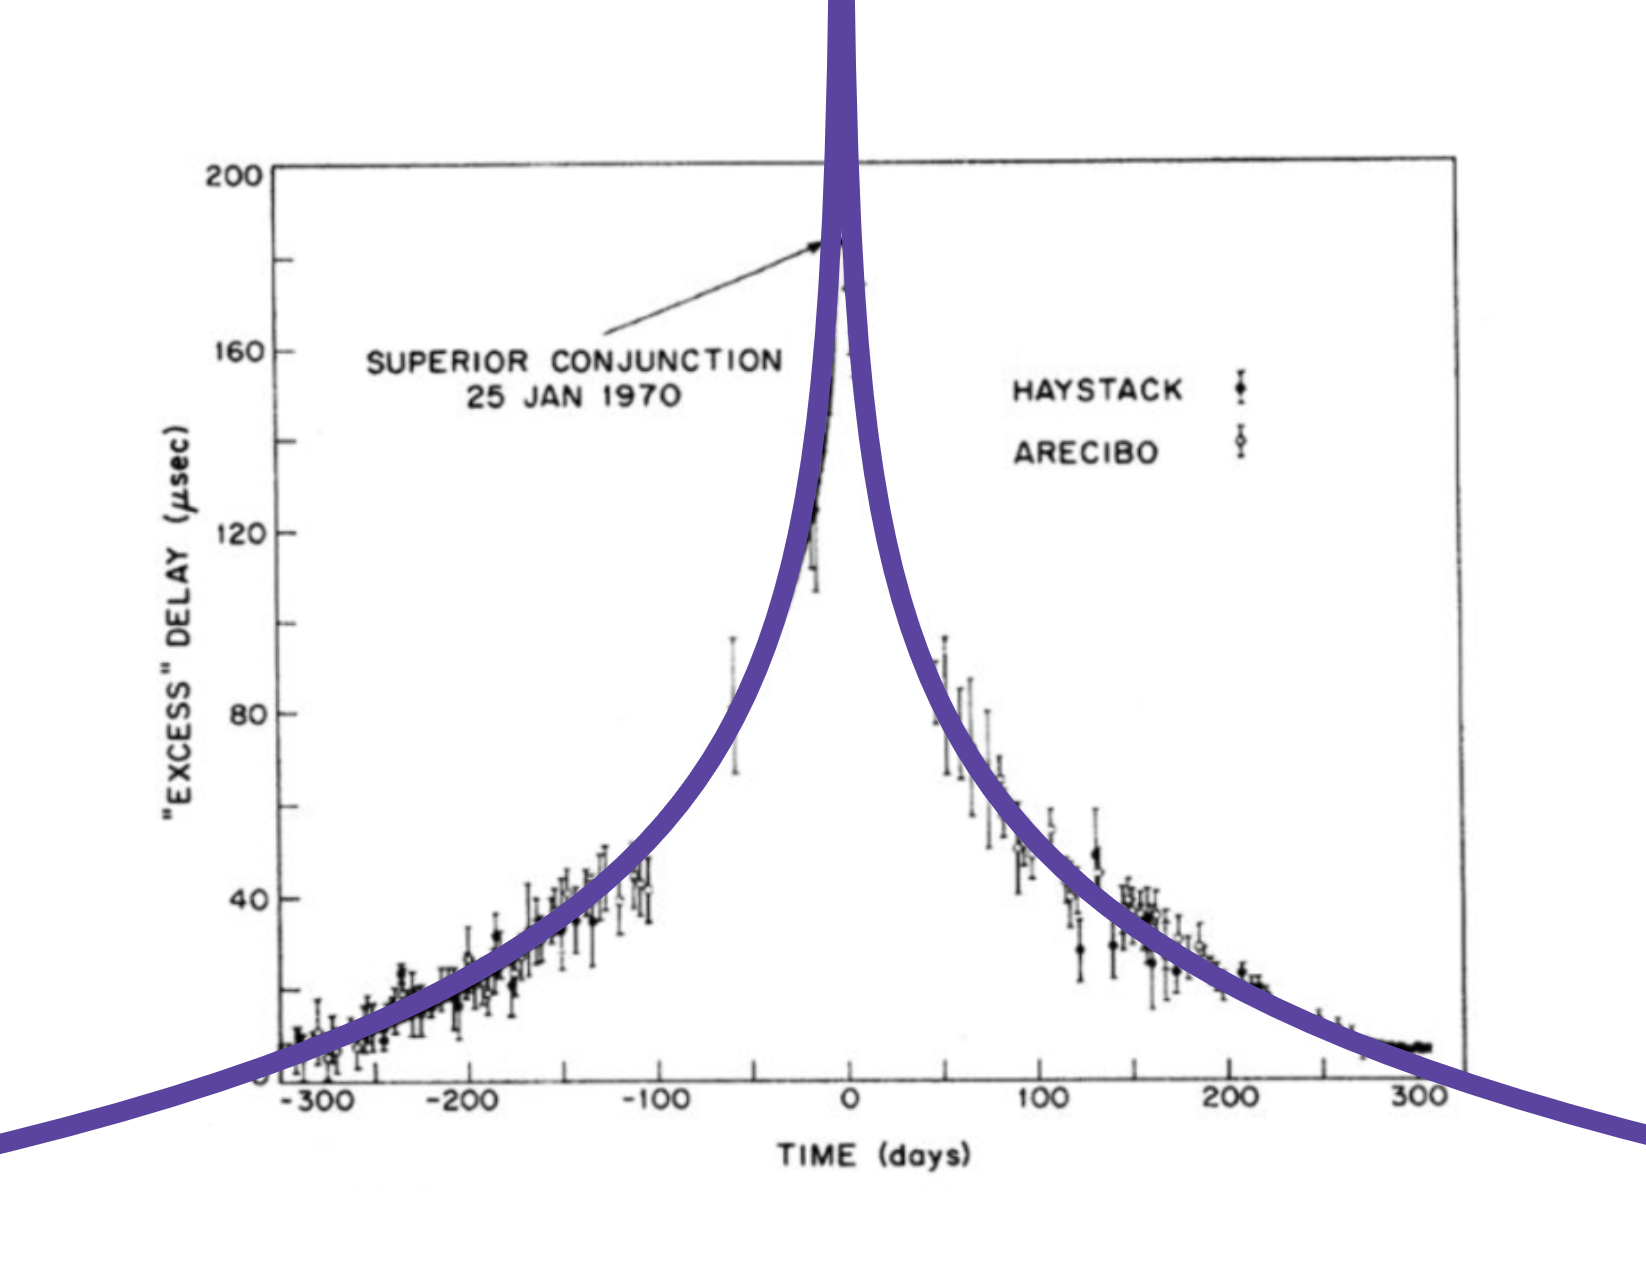
\includegraphics[scale=0.5]{timedelay.png}
  \end{center}
  If we assume that the radius of closest approach $r_0$ varies linearly with time around the point of superior conjunction, this is strong evidence that our derived time delay function is at least of the right form. To verify this quantitatively, we would need more information about the geometry of the Earth, the sun, and Venus to compute exact values for $r_A$, $r_B$, and $r_0$.
\end{parts}

\end{document}

